\chapter{Apprendimento Bayesiano}
In questo capitolo considereremo l'apprendimento come una forma di ragionamento incerto sulle osservazioni. Sappiamo che l'incertezza è prevalente negli ambienti reali e gli agenti possono gestirla mediante metodi probabilistici. Per far ciò però essi devono apprendere una loro teoria probabilistica del mondo circostante. Il punto di vista Bayesiano sull'apprendimento è estremamente potente ed offre soluzioni generali ai problemi del rumore, del sovradattamento e della predizione ottima. Viene anche considerato il fatto che un agente non onnisciente non potrà mai essere certo della correttezza di una teoria sul mondo ma deve comunque utilizzarne una per prendere delle decisioni, per cui viene sfruttata \textbf{solitamente} l'ipotesi più probabile. Nell'ambito Bayesiano si cambia l'approccio avendo la valutazione d'ipotesi in base alla loro probabilità. Si studia la probabilità rispetto ai dati e rispetto alle conoscenze pregresse. Non troviamo quindi un'ipotesi perfettamente compatibile ma una che è più probabile rispetto ad altre. Bisogna dunque studiare come scegliere le ipotesi, usando risultati noti del calcolo
probabilistico. Useremo le nozioni di probabilità e probabilità condizionata, oltre ovviamente alla \textbf{regola di Bayes}.
Si assume quindi che le quantità d'interesse siano ``governate'' da
distribuzioni di probabilità e che la decisione migliore può essere presa ragionando su tali distribuzioni e sull'insieme di dati di
training. L'apprendimento Bayesiano è importante per due ragioni principali:
\begin{enumerate}
  \item si ha una manipolazione esplicita delle probabilità rispetto ad altri approcci pratici di alcuni tipi di problemi di apprendimento (infatti si hanno
  spesso paragoni con gli alberi decisionali e con le reti neurali)
  \item fornisce una prospettiva utile per comprendere metodi di apprendimento
  che non manipolano effettivamente le probabilità
\end{enumerate}
\section{Apprendimento Statistico}
I concetti chiave sono i \textbf{dati} e le \textbf{ipotesi}. I dati rappresentano \textbf{prove}, ovvero istanziazioni di alcune o tutte le \textbf{\href{https://it.wikipedia.org/wiki/Variabile_casuale}{Variabili Casuali}} che descrivono il dominio. Le ipotesi invece esprimono  teorie probabilistiche sul funzionamento del dominio.
Dal punto di vista delle funzionalità si ha che ogni esempio di training osservato può aumentare o diminuire, in modo incrementale, la stima di probabilità relativa alla correttezza di un'ipotesi. Inoltre, come già anticipato, la conoscenza pregressa può essere combinata con i dati osservati per determinare la probabilità finale delle varie ipotesi. In particolare si afferma inoltre che le
varie ipotesi possono effettuare predizioni probabilistiche e le istanze possono essere quindi classificate combinando le predizioni delle varie ipotesi, che sono pesate tramite il peso delle loro probabilità. Con il metodo Bayesiano si ottiene quindi uno ``standard'' per prendere decisioni ottimali rispetto al quale è possibile misurare ulteriori misure pratiche.\\
Si hanno però alcune difficoltà legate all'apprendimento Bayesiano:
\begin{itemize}
  \item si necessita avere la conoscenza di varie probabilità
  \item si hanno costi computazionali non indifferenti
\end{itemize}
\subsection{Probabilità a priori delle ipotesi e Verosimiglianza}
\begin{definizione}[Apprendimento Bayesiano]
L'apprendimento Bayesiano calcola semplicemente la probabilità di ogni ipotesi condizionandola ai dati osservati,  e su tale base formula predizioni. Le predizioni possono essere quindi basate su tutte le ipotesi, pesate secondo la rispettiva probabilità, e non solo su quella migliore.
\end{definizione}
% Inquadrando nuovamente il fulcro del machine learning ricordiamo che si sta
% cercando la ``miglior'' ipotesi $h$, contenuta dello spazio delle ipotesi $H$, a
% partire dai dati contenuti in un training set $D$. Nell'apprendimento Bayesiano
% si ha che la ``miglior'' ipotesi altro non è che la più probabile. Ovviamente
% potrebbero esistere più ipotesi. 
La \textbf{formula di Bayes} fornisce un metodo diretto per calcolare la probabilità di tale ipotesi in base:
\begin{itemize}
  \item alla sua probabilità conosciuta a priori
  \item alle probabilità di osservare vari dati data l'ipotesi
  \item ai dati stessi
\end{itemize}
\begin{definizione}[Definizione di Bayes]
  Preso il DataSet \textbf{d}, allora definiamo la distribuzione di probabilità a \textbf{posteriori}:
  \[P(h_i|d)=\frac{P(d|h_i)P(h_i)}{P(d)}\]
  Dove:
  \begin{itemize}
        \item $P(h_i)$ viene chiamata \textbf{probabilità a priori delle ipotesi}
        \item $P(d|h_i)$ è la \textbf{verosimiglianza} dei dati sotto ogni ipotesi.
        \item $P(d)$ che è la probabilità conosciuta a priori di del dataset, ovvero la
     probabilità che esso sia osservato.\\ Si calcola come: $P(d)=\sum_i(d, h_i)=\sum_i P(d|h_i)P(h_i)$
    \end{itemize}
%   \begin{itemize}
%     \item $P(h)$ che è la probabilità conosciuta a priori di $h$. Tale
%     probabilità riflette qualsiasi conoscenza di base sulla possibilità
%     che $h$ sia corretta  
%     \item $P(d)$ che è la probabilità conosciuta a priori di $D$, ovvero la
%     probabilità che $D$ sia osservato
%     \item $P(d|h)$ che è la probabilità di osservare $D$ in presenza
%     dell'ipotesi $h$
%     \item $P(h|d)$ che è la probabilità a posteriori di $h$. Tale probabilità
%     riflette la ``confidenza'' di avere $h$  dopo che $D$ è stato osservato
%   \end{itemize}
\end{definizione}
\begin{definizione}
Sia \textbf{D} il DataSet dove i valori osservati vengono indicati con \textbf{d}. Supponiamo di voler predire una predizione $"X"$:
\begin{equation}
    P(X|d)=\sum_{i}P(X|d, h_i)P(h_i|d) = \sum_{i}P(X|h_i)P(h_i|d) 
    \label{Bayes}
\end{equation}
\begin{nota}
    Abbiamo presunto che ogni ipotesi determini una distribuzione di probabilità $X$. Quest'equazione mostra che le predizioni sono medie pesate delle predizioni delle singole ipotesi. Le ipotesi stesse fungono essenzialmente da \textit{intermediari} tra i dati nudi e le predizioni.
\end{nota}
\end{definizione}
La figura \ref{fig:Prob2} mostra la predizione della probabilità che l'osservazione successiva abbia una data classificazione, seguendo la \ref{Bayes}. 
\begin{figure}[H]
    \centering
    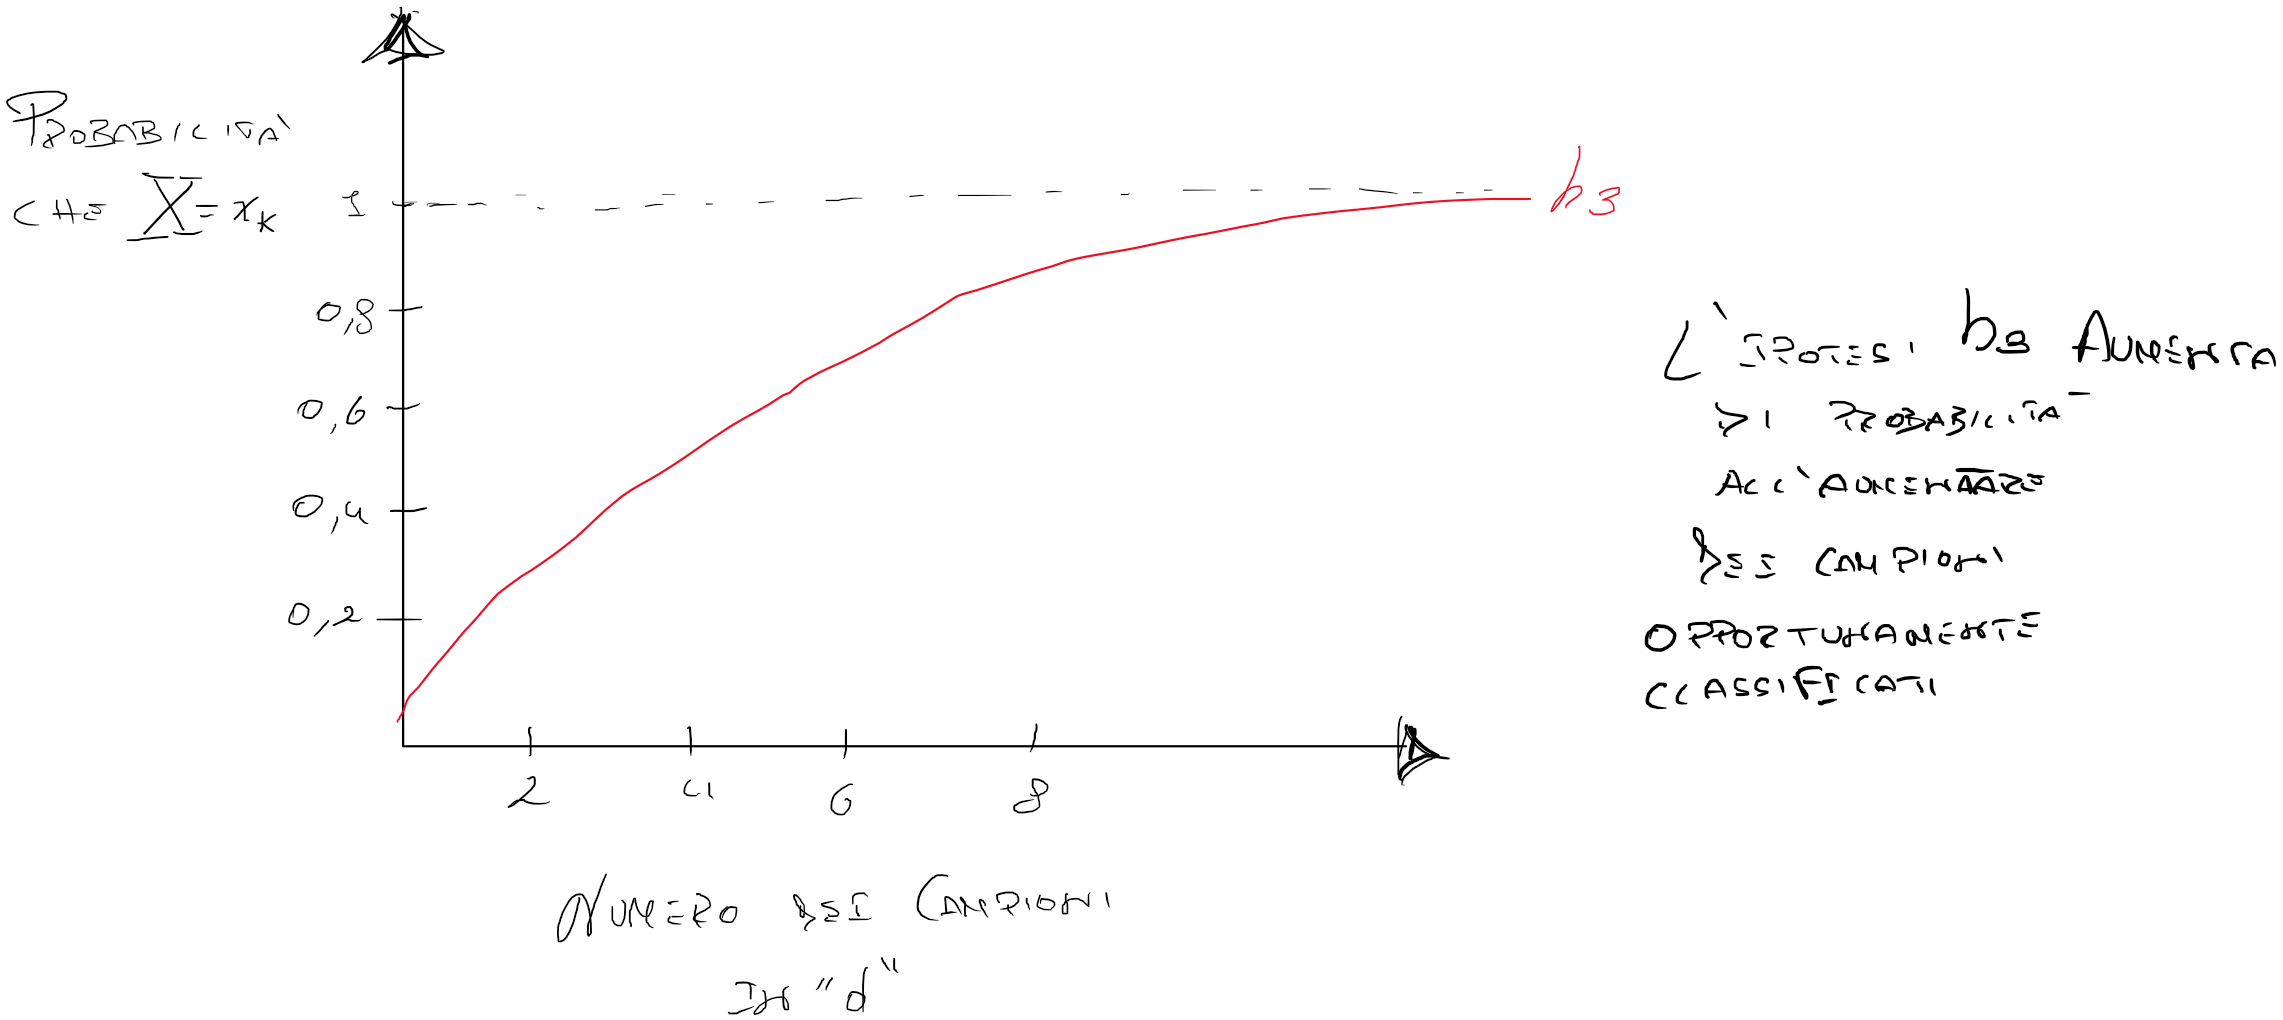
\includegraphics[width=1\textwidth]{img/prob2.png}
    \caption{Predizione bayesiana $P(d_{n+1} = x_k | d1 \dots d_n)$}
    \label{fig:Prob2}
\end{figure}
\begin{definizione}[Verosimiglianza]
  La verosimiglianza dei dati è calcolata partendo dal presupposto che le osservazioni $d_j$ in un dataset \textbf{d}, siano indipendentemente e identicamente distribuite (\textbf{i.i.d}), così che:
  \[P(d|h_i)=\prod_{j}P(d_j|h_i)\]
\end{definizione}
La figura \ref{fig:Prob1} mostra come cambia la probabilità a posteriori di alcune ipotesi man mano che viene osservata una sequenza di elementi in \textbf{d}.
\begin{figure}[H]
    \centering
    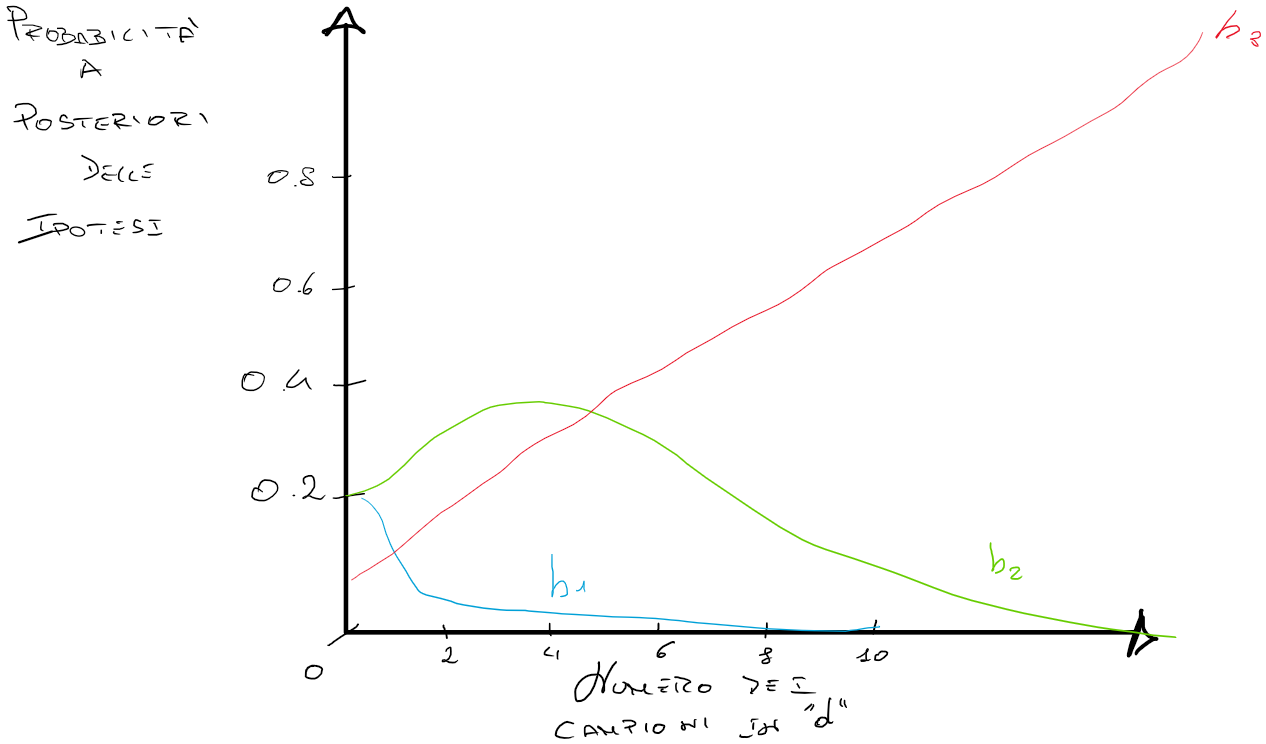
\includegraphics[width=1\textwidth]{img/prob1.png}
    \caption{Predizione delle ipotesi al variare dei campioni correttamente predetti.}
    \label{fig:Prob1}
\end{figure}
\subsection{Massima a posteriori}
La predizione bayesiana è \textbf{ottima}, indipendentemente dalle dimensioni dell'insieme dei dati: in altre parole, sarà corretta più spesso di qualsiasi altra predizione. Naturalmente c'è un prezzo da pagare per l'ottimalità dell'apprendimento bayesiano. Difatti nei sistemi reali i dati da gestire sono molti e spesso si deve ricorrere forzatamente ad una qualche forma ti approssimazione. \\ 
Un'approssimazione molto comune è formulare predizioni che si basano su un'ipotesi più probabile: la $h_i$ che massimizza $P(h_i| d)$. Questa viene spesso denominata \textbf{massimo a posteriori} o MAP. Le predizioni che si basano su un'ipotesi $h_{MAP}$ sono approssimativamente bayesiane dal momento che:
\[P(X|d) \approx P(X|h_{MAP})\]
La figura \ref{fig:Prob1} mostra difatti che l'ipotesi $h_2 = h_{MAP}$ dopo un certo numero di classificazioni tali per cui $d_{n+1} = x_k$ (ovvero dopo aver predetto una certa sequenza di classificazioni), per cui un agente MAP predirà che l'\textit{n-esimo} valore sarà opportunamente classificato con $x_k$ con probabilità 1. 
Man mano che vengono elaborati nuovi dati, la predizione MAP e quella bayesiana si avvicinano (dato che le altre predizioni "candidate" MAP diventano meno probabili). Generalmente trovare l'ipotesi MAP è più facile poiché si sta risolvendo un problema di ottimizzazione anziché eseguire una grande sommatoria.
\begin{definizione}
  Definiamo le \textit{ipotesi maximum a posteriori (MAP)} ogni ipotesi
  massimamente probabile:
  \[h_{MAP}=\operatorname*{argmax}_{h\in H}P(h|d)\]
  \[\operatorname*{argmax}_{h\in H}\frac{P(d|h)P(h)}{P(d)}\]
  Ma $P(d)$ può essere cancellato in quanto costante e indipendente da $h$,
  ottenendo:
  \[h_{MAP}=\operatorname*{argmax}_{h\in H}P(d|h)P(h)\]
\end{definizione}
\subsection{Massima Verosimiglianza}
Un'ultima semplificazione si può ottenere presupponendo una distribuzione a priori uniforme dello spazio delle ipotesi. Spesso si assume anche che ogni ipotesi è, a priori, equiprobabile e quindi possiamo semplificare i conti. La massima verosimiglianza (maximum likehood) si indica con ML. Esso è un approccio ragionevole quando non c'è ragione di preferire a priori un'ipotesi all'altra.
\begin{definizione}
  Dato che $P(d|h)$ viene spesso chiamata \textbf{likehood
    (\textit{probabilità})} di $D$ data $h$ viene definita \textbf{ipotesi
    maximum likehood (ML)} ogni ipotesi che massimizza $P(d|h)$:
  \[h_{ML}=\operatorname*{argmax}_{h\in H}P(d|h)\]
  potendo quindi trascurare $P(h)$ in quanto equivalente $\forall\, h\in H$
\end{definizione}
\subsubsection{Learn a Read-Value Function}
Ipotizziamo di voler trovare un'ipotesi per una funzione target:
\begin{figure}[H]
    \centering
    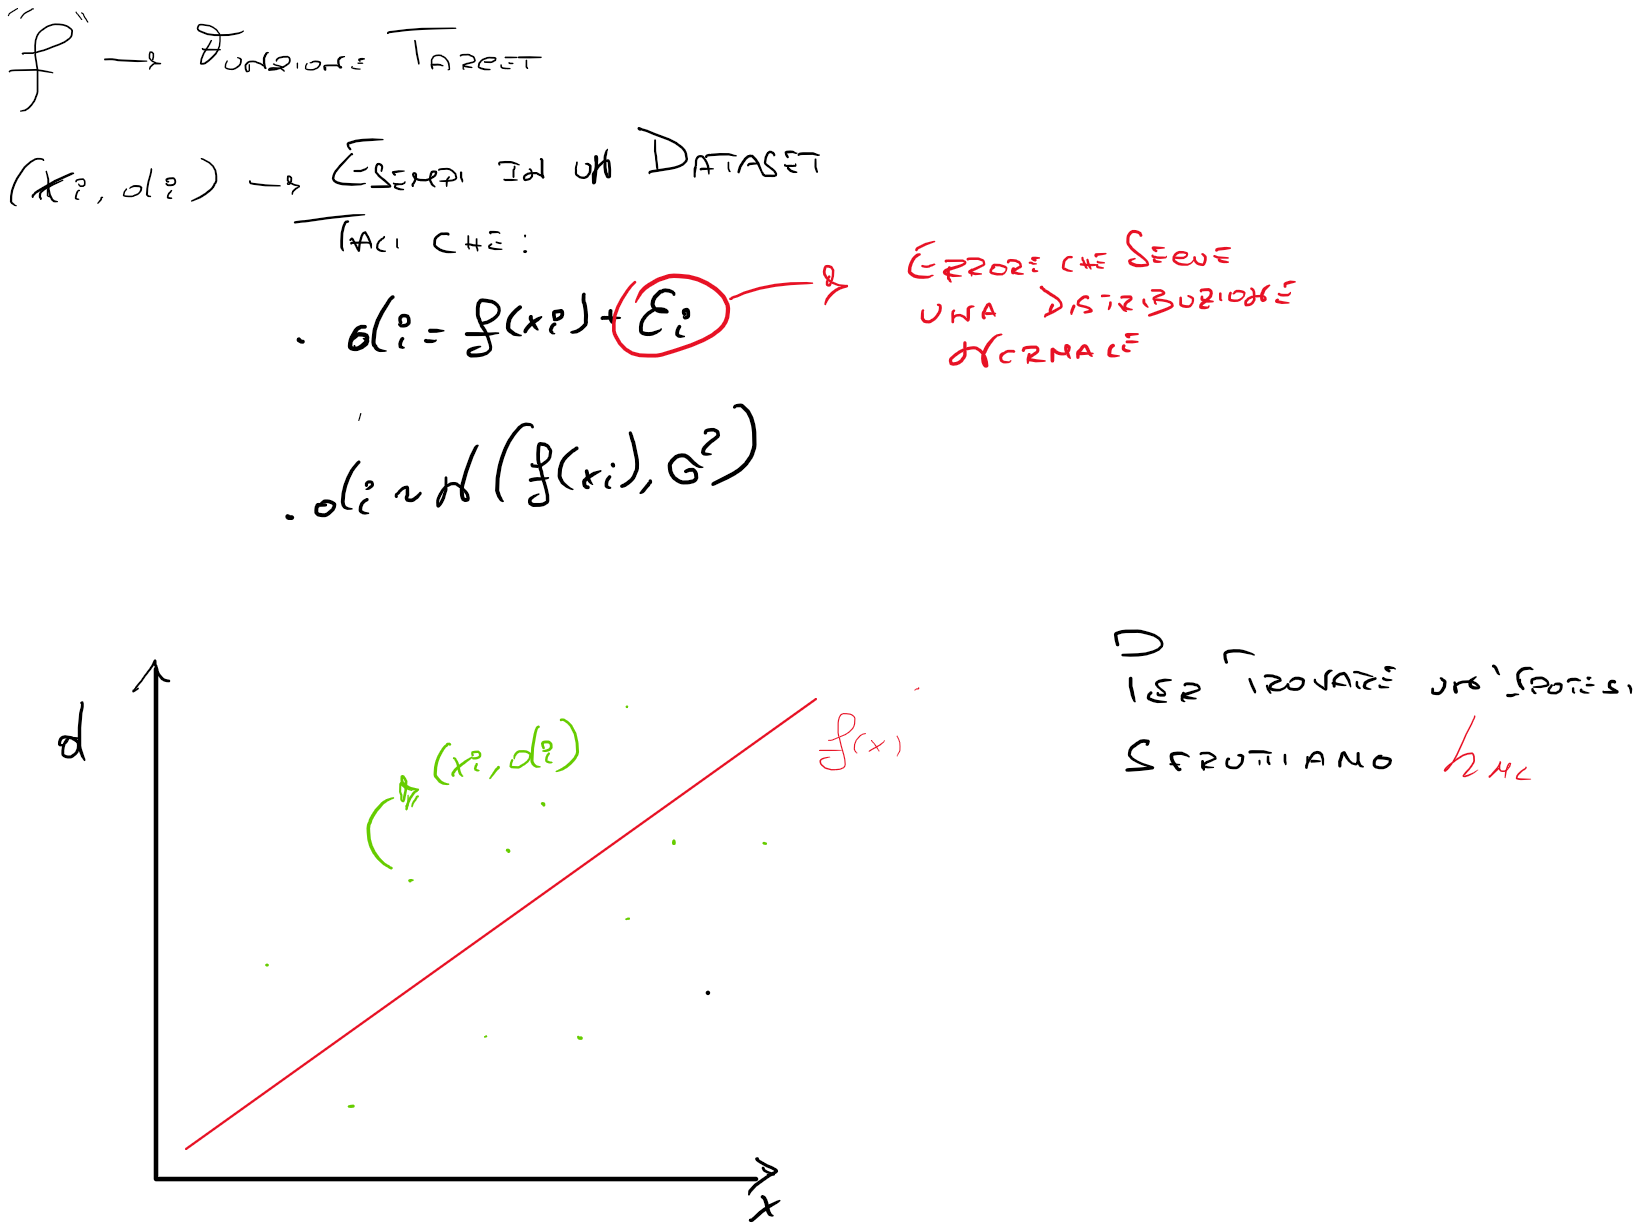
\includegraphics[width=1\textwidth]{img/hml.png}
\end{figure}
Avendo quindi che $h_{ML}=\operatorname*{argmax}_{h\in H}P(d|h)$ e che gli
eventi di training vengono assunti come indipendenti si ha che:
\[h_{ML}=\operatorname*{argmax}_{h\in H}\prod_{i=1}^mP(d_i|h) = \operatorname*{argmax}_{h\in H}P(d|h) \]
Dato quindi l'errore e$_i$ distribuito normalmente con media zero e varianza
sconosciuta $\sigma^2$ si ha che anche ogni $d_i$ segue la stessa
distribuzione attorno al target $f(x_i)$. Poiché stiamo scrivendo l'espressione
per $P(d|h)$, assumiamo che $h$ sia la descrizione corretta per $f$, quindi:
\[\mu=f(x_i)=h(x_i)\]
e avendo quindi, per la distribuzione normale:
\[h_{ML}=\operatorname*{argmax}_{h\in H}
  \prod_{i=1}^m\frac{1}{\sqrt{2\pi\sigma^2}}
  e^{-\frac{1}{2\sigma^2}(d_i-h(x_i))^2}\]
È comune massimizzare il logaritmo meno complicato, a causa della monotonia di
questa funzione, avendo:
\[h_{ML}=\operatorname*{argmax}_{h\in
    H}\prod_{i=1}^m\frac{1}{\sqrt{2\pi\sigma^2}}
  -\frac{1}{2\sigma^2}(d_i-h(x_i))^2\]
ma il primo termine è costante e indipendente da $h$ e quindi può essere
cancellato:
\[h_{ML}=\operatorname*{argmax}_{h\in
    H}\prod_{i=1}^m -\frac{1}{2\sigma^2}(d_i-h(x_i))^2\]
Sapendo che massimizzare questo termine negativo equivale a ridurre al minimo il
termine positivo corrispondente:
\[h_{ML}=\operatorname*{argmin}_{h\in
    H}\prod_{i=1}^m \frac{1}{2\sigma^2}(d_i-h(x_i))^2\]
e avendo che anche tutte le costanti sono indipendenti da $h$ e quindi possono
essere rimosse:
\[h_{ML}=\operatorname*{argmin}_{h\in H}\prod_{i=1}^m (d_i-h(x_i))^2\]
trovando che $h_{ML}$ è ciò che minimizza gli errori quadratici. \\
Si specifica la scelta della normale in quanto:
\begin{itemize}
  \item buona approssimazione di molti tipi di rumore nei sistemi fisici 
  \item il definizione del Limite Centrale mostra che la somma di un numero
  sufficientemente grande di variabili casuali indipendenti e identicamente
  distribuite obbedisce a una distribuzione Normale 
\end{itemize}
\textbf{\textit{Si considera solo il rumore sul valore del target e non sugli
    attributi che descrivono le istanze stesse}}.
% \subsection{Brute-Force MAP LEARNING}
% Si può usare il definizione di Bayes per specificare un algoritmo di apprendimento
% molto semplice detto \textbf{algoritmo Brute-Force MAP LEARNING} che si articola
% in 2 step:
% \begin{enumerate}
%   \item $\forall\, h\in H$ calcolo la probabilità a posteriori tramite il definizione
%   di Bayes:
%   \[P(h|d)=\frac{P(d|h)P(h)}{P(d)}\]
  
%   \item restituisco l'ipotesi $h_{MAP}$ con la più alta probabilità a
%   posteriori:
%   \[h_{MAP}=\operatorname*{argmax}_{h\in H}P(h|d)\]
% \end{enumerate}
% Però, per specificare il problema d'apprendimento per l'algoritmo, bisogna
% obbligatoriamente specificare i valori di:
% \begin{itemize}
%   \item $P(h)$
%   \item $P(d|h)$
% \end{itemize}
% e quindi dobbiamo obbligatoriamente fare una serie di assunzioni:
% \begin{itemize}
%   \item il training set deve essere privo di rumore, avendo:
%   \[d_i=c(x_i)\]
%   \item il target concept deve essere contenuto nello spazio delle ipotesi:
%   \[\exists h\in H \mbox{t.c. }h(x)=c(x),\,\,\,\forall\, x\in X\]
%   \item devo assumere che le ipotesi siano equiprobabili e quindi:
%   \[P(h)=\frac{1}{|H|}\,\,\,\forall\, h\in H\]
%   e avendo quindi:
%   \[P(d|h)=
%     \begin{cases}
%       1&\mbox{se } d_i=h(x_i),\,\,\,\forall\, d_i\in D\\
%       0&\mbox{altrimenti}
%     \end{cases}
%   \]
% \end{itemize}
% Si ha quindi che il problema di apprendimento per l'algoritmo è completamente
% definito. Possiamo quindi specificare che, nel primo step, ovvero quando si
% cerca $P(h|d)$, posso avere due casi:
% \begin{enumerate}
%   \item $h$ è inconsistente con $D$, avendo quindi:
%   \[P(h|d)=\frac{0\cdot P(h)}{P(d)}=0\]
%   \item $h$ è consistente con $D$, avendo quindi:
%   \[P(h|d)=\frac{1\cdot \frac{1}{|H|}}{P(d)}=\frac{1\cdot
%       \frac{1}{|H|}}{\frac{|VS_{H, D}|}{|H|}}=\frac{1}{|VS_{H, D}|}\] 
% \end{enumerate}
% Si ha quindi che questa analisi implica che, sotto le condizioni sopra definite,
% ogni ipotesi coerente è un'ipotesi MAP, perché per ogni ipotesi coerente si ha
% che:
% \[P(h|d)=\frac{1}{|VS_{H, D}|}\]
% \begin{figure}
%   \centering
%   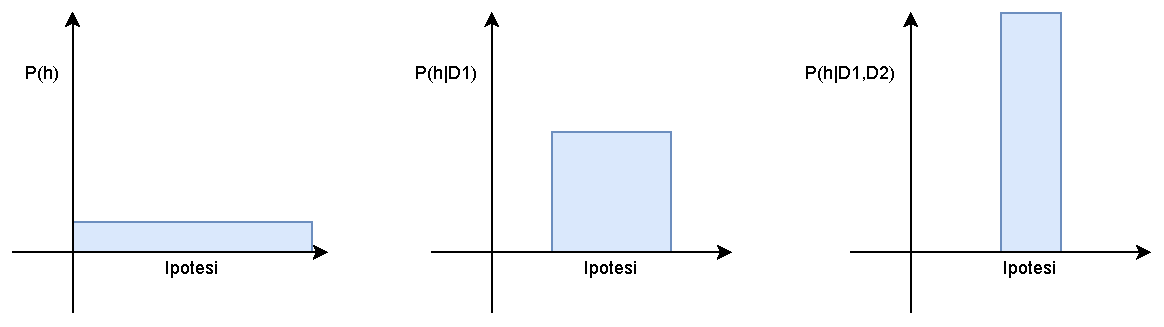
\includegraphics[scale = 0.6]{img/map.pdf}
%   \caption{Nell'immagine le evoluzioni di probabilità delle
%     ipotesi. Nel primo grafico tutte le ipotesi hanno la stessa probabilità, è
%     il punto di partenza. Con gli altri due grafici si ha che man mano che i
%     dati di addestramento si accumulano, la probabilità a posteriori delle
%     ipotesi inconsistenti diventa zero mentre la probabilità totale che si somma
%     a 1 è condivisa equamente tra le ipotesi consistenti rimanenti.}
% \end{figure}
% Si ha che ogni learner consistente ha in output ipotesi MAP se si assume a
% priori la distribuzione uniforme delle probabilità su $H$ dati di training
% deterministici e privi di rumore.\\
% Riprendendo per esempio anche l'algoritmo find-S si ha che:
% \begin{itemize}
%   \item ha in output ipotesi consistenti e quindi ipotesi MAP sotto la
%   distribuzione di probabilità $P(h)$ e $P(d|h)$
%   \item $\forall\, P(h)$ che favorisce le ipotesi più specifiche find-S trova
%   appunto le ipotesi MAP
% \end{itemize}
% A riprova che il metodo Bayesiano è un modo per caratterizzare il comportamento
% degli algoritmi di apprendimento.\\
% inoltre, identificando $P(h)$ e $P(d|h)$ base alle quali l'output è l'ipotesi
% ottimale, è possibile caratterizzare le ipotesi implicite dell'algoritmo ovvero
% il \textbf{bias induttivo} dell'algoritmo (avendo anche che l'inferenza
% induttiva è modellata da un sistema di ragionamento probabilistico equivalente
% basato sulla definizione di Bayes). \\
% Si introduce ora il problema di apprendere funzioni target a valori continui
% (reti neurali regressione lineare etc$\ldots$). Si ha che in base a determinate
% ipotesi, qualsiasi algoritmo di apprendimento che minimizzi l'errore quadratico
% tra l'ipotesi di output e i dati di addestramento, produrrà un'ipotesi
% ML. Prepariamo quindi il nostro insieme di assunzioni per il problema:
% \begin{itemize}
%   \item $h:X\to\mathbb{R},\,\,\,\forall\, h\in H$
%   \item li esempi sono della forma $\langle x_i, d_i\rangle$
%   \item la funzione target è definita come $f:X\to\mathbb{R}$
%   \item si hanno $m$ esempi di training dove il valore target di ogni esempio è
%   ``sporcato'' dal rumore casuale $e_i$ secondo una distribuzione di probabilità
%   normale con media nulla, avendo $d_i=f(x_i)+e_i$
% \end{itemize}
\subsection{Minima Lunghezza della descrizione}
Sia nell'apprendimento bayesiano che in quello MAP la distribuzione a priori delle ipotesi $P(h_i)$ ha un ruolo importante difatti ha il ruolo di \textit{penalizzare la complessità} nel caso di \textbf{overfitting}. Tipicamente le ipotesi più complesse hanno una probabilità a priori più bassa, sebbene abbiano una maggior capacità di adattarsi ai dati. Quindi la probabilità a priori rappresenta un compromesso tra la sua complessità e la sua capacità di adattarsi ai dati.
Anche in questo caso si usa il Rasoio di Occam, scegliendo di usare il principio
\textbf{Minimum Description Length (\textit{MDL})}, scegliendo la spiegazione
più breve per i dati osservati.\\
Tramite MDL posso ``giustificare'' la scelta di $h_{MAP}$ in base alla teoria
dell'informazione, infatti:
\[h_{MAP}=\operatorname*{argmax}_{h\in H}P(d|h)P(h)\]
\[=\operatorname*{argmax}_{h\in H}\log_2P(d|h)+\log_2P(h)\]
\[=\operatorname*{argmin}_{h\in H}-\log_2P(d|h)-\log_2P(h)\]
e queste equazioni possono essere interpretate come un'affermazione che sono
preferite ipotesi brevi, assumendo un particolare schema di rappresentazione per
la codifica d'ipotesi e dati.\\
Il principio MDL fornisce un modo per scambiare la complessità delle ipotesi
per il numero di errori commessi dall'ipotesi.\\

\textbf{Su slide altre informazioni su teoria dell'informazione.}
\section{Classificatore Bayesiano ottimo}
Ci si chiede quindi qual è la \textbf{classificazione più probabile} della nuova istanza
secondo i dati di training.\\
Vediamo con un esempio che non basta applicare $h_{MAP}$:
\begin{esempio}
  Sia $H=\{h_1, h_2, h_3\}$ con $P(h_1)=0.4$ e $P(h_2)=P(h_3)=0.3$.\\
  Si ha quindi che:
  \[h_{MAP}=h_1\]
  Consideriamo però una nuova istanza $x$ classificata positiva per $h_1$ e
  negativa per le altre due. Si ha quindi che:
  \begin{itemize}
    \item la probabilità che $x$ sia positivo è 0.4
    \item la probabilità che $x$ sia negativo è 0.6
  \end{itemize}
  e quindi la classificazione più probabile non è quella di $h_{MAP}$.
\end{esempio}
Abbiamo che la classificazione più probabile si ottiene combinando le previsioni
di tutte le ipotesi, ponderate in base alle loro probabilità posteriori. Data
$P(X|d)$ come la probabilità che la classificazione corretta sia $X$:
\[P(X|d)=\sum_{h_i\in H}P(X|h_i)P(h_i|d)\]
ottenendo che il classificatore Bayesiano ottimo è:
\[\operatorname*{argmax}_{X\in V}\sum_{h_i\in H}P(X|h_i)P(h_i|d)\]
dato $V$ come insieme di tutte le possibili predizioni esistenti.
\begin{esempio}
  Vediamo un esempio chiarificatore.\\
  Sia $V=\{+,-\}$ e siano:
  \begin{itemize}
    \item $P(h_1, d) =0.4,\,\,\, P(-, h_1) = 0,\,\,\, P(+, h_1) = 1$
    \item $P(h_2, d) =0.3,\,\,\, P(-, h_2) = 1,\,\,\, P(+, h2) = 0$
    \item $P(h_3, d) =0.3,\,\,\, P(-, h_3) = 1,\,\,\, P(+, h3) = 0$
  \end{itemize}
  Si hanno:
  \[\sum_{h_i\in H}P(+|h_i)P(h_i|d)=0.4\]
  \[\sum_{h_i\in H}P(-|h_i)P(h_i|d)=0.6\]
  \[\operatorname*{argmax}_{X\in \{+,-\}}\sum_{h_i\in H}P(X|h_i)P(h_i|d)= - \]
\end{esempio}
\section{Classificatore Bayesiano naive}
Il modello di rete bayesiana più usato nell'apprendimento automatico è probabilmente quello  \textbf{bayesiano ingenuo/naive}. Tale nomenclatura è data poiché il modello presume che gli attributi siano tutti condizionalmente indipendenti l'uno dall'altro, data la classe.
Il Classificatore Bayesiano naive si applica alle attività di learning in
cui ogni istanza $x$ è descritta da una giunzione di valori di attributi e in
cui la funzione target $f(x)$ può prendere un valore qualsiasi dall'insieme
finito $V$. Descriviamo gli esempi di training come $\langle d_1, d_2,\ldots
d_n\rangle $. \\
Applicando il metodo Bayesiano si ha:
\[h_{MAP}=\operatorname*{argmax}_{h\in V}P(h|d_1, d_2,\ldots d_n)\]
\[=\operatorname*{argmax}_{h\in V}\frac{P(d_1, d_2,\ldots d_n|h)P(h)}{P(d)}\]
e, rimuovendo le i fattori indipendenti:
\[h_{MAP}=\operatorname*{argmax}_{h\in V}P(d_1, d_2,\ldots d_n|h)P(h)\]
Avendo che:
\begin{itemize}
  \item $P(h)$ può essere stimato tramite la frequenza di $h$ in $D$
  \item $P(d_1, d_2,\ldots d_n|h)$ non può essere stimato in questo modo ma il
  numero di questi termini è pari a $|X|\cdot |V|$
\end{itemize}
Con il classificatore Bayesiano naive si hanno diverse semplificazioni. In primis
i valori degli attributi sono condizionatamente indipendenti:
\begin{itemize}
  \item $P(d_1, d_2,\ldots d_n|h)=\prod_iP(d_i|h)$
  \item il numero dei termini $d_1, d_2,\ldots d_n$ è pari a:
  \[|DA|\cdot |DT|+|DT|\]
  ove:
  \begin{itemize}
    \item $DA$ sta per attributi distinti/unici
    \item $DT$ sta per valori di target distinti/unici
  \end{itemize}
  \item non si ha la ricerca esplicita dentro $H$ ma solo il contro delle
  frequenze 
\end{itemize}
Si ha quindi il classificatore Bayesiano naive:
\[v_{NB}=\operatorname*{argmax}_{h\in V}P(h)\prod_iP(d_i|h)\]
\newpage
\begin{esempio}
  Vediamo un esempio chiarificatore.\\
  Sia dato il seguente dataset, con il target \textit{PlayTennis}:
  \begin{figure}[H]
    \centering
\    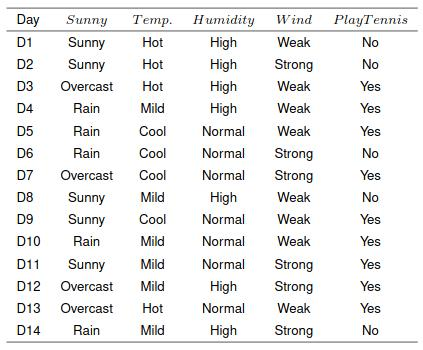
\includegraphics[scale = 0.7]{img/cbn.jpg}
  \end{figure}
  Si ha la nuova istanza:
  \[\langle Outlook=Sunny, Temperature=Cool, Humidity=High,
      Wind=Strong \rangle\]
  Si ha quindi che:
  \[\prod_iP(a_i|h)=(Outlook=sunny|h)\cdot
      P(Temperature=cool|h)\]\[\cdot P(Humidity=high|h)\cdot
      P(Wind=strong|h)\]
 
  Avendo la stima delle probabilità:
  \[P(PlayTennis=yes)=\frac{9}{14}=0.64\]
  \[P(PlayTennis=no)=\frac{5}{14}=0.36\]
  In modo analogo calcolo le probabilità condizionali. Per esempio per
  $Wing=Strong$:
  \[P(Wing=Strong|PlayTennis=yes)=\frac{3}{9}=0.33\]
  \[P(Wing=Strong|PlayTennis=no)=\frac{3}{5}=0.60\]
  Posso quindi calcolare $v_{NB}$:
  \[P(yes)\cdot P(Sunny|yes)\cdot P(cool|yes)\cdot P(high|yes)\cdot
    P(cool|yes)=0.0053\]
  \[P(no)\cdot P(Sunny|no)\cdot P(cool|no)\cdot P(high|no)\cdot
    P(cool|no)=0.0206\]
  Quindi si ha che:
  \[v_{NB}=no\]
  e normalizzando:
  \[\frac{0.0206}{0.0206+0.0053}\]
\end{esempio}
Si è visto come, normalmente, le probabilità sono stimate dalla frazione di
volte in cui si osserva che l'evento si verifica sul numero totale di
opportunità $N$:
\[\frac{n_c}{N}\]
è spesso questo metodo fornisce una buona stima.\\
Si ha però un limite se $n_c$ è molto piccolo, avendo risultati errati con:
\begin{itemize}
  \item sottovalutazione delle probabilità a causa di un bias
  \item se addirittura $n_c$ è nullo esso ``dominerà'' sul classificatore
  Bayesiano 
\end{itemize}
Si introduce un nuovo approccio Bayesiano sfruttando il cosiddetto
\textbf{m-estimate}, ovvero: 
\[\frac{n_c+m\cdot p}{n+m}\]
dove $p$ è una stima precedente della probabilità che desideriamo determinare,
ed $m$ è una costante chiamata \textit{equivalent sample size} che determina
quanto sia importante il peso di $p$ rispetto ai dati osservati.\\
In assenza d'informazioni aggiuntive $p$ ha distribuzione uniforme quindi si
ha, per $k$ numero di possibili valori di attributo:
\[p=\frac{1}{k}\]
Si nota che per $m$ nullo si ha che l'm-estimate è uguale a:
\[\frac{n_c}{n}\]
e quindi $m$ può essere interpretato come il numero di campioni virtuali
distribuiti su $p$ a cui vengono aggiunti gli $n$ esempi effettivi osservati.
\section{Esempi}
Si ricorda che si cerca una strategia per trovare la miglior ipotesi nello
spazio delle ipotesi. In questo caso si parla di ``migliore'' in termini di più
``probabile''. \\
Quando si fa inferenza bayesiana è tutto governato da \textit{incertezza} ma
permette di sfruttare conoscenze a priori.\\
Ricordiamo quindi la formula di Bayes:
\[P(h|d)=\frac{P(d|h)P(h)}{P(d)}\]
con:
\begin{itemize}
  \item $D$ è il dataset
  \item $h$ che per noi è l'ipotesi
  \item $P(h|d)$ che è la distribuzione a posteriori
  \item $P(h)$ è la distribuzione a priori
  \item $P(d|h)$ è la verosimiglianza
  \item $P(d)$ è l'evidenza
\end{itemize}
Sapendo che:
\[P(d)=\sum_i(d, h_i)=\sum_i P(d|h_i)P(h_i)\]
$P(d)$ è invariante rispetto al valore dell'ipotesi e quindi possiamo benissimo
rimuoverlo nel calcolo in quanto non influisce sulla probabilità a posteriori:
\[P(h_i|d)\varpropto P(d|h_i)P(h_i)\]
\begin{nota}
    Si ricorda che $\varpropto$ indica "\textit{proposizionale a}" quindi che due
cose sono uguali al più di una costante.
\end{nota}
Ricordiamo inoltre che la massima ipotesi a posteriori è:
\[h_{MAP}=\operatorname*{argmax}_{h\in H}P(h|d)=
  \operatorname*{argmax}_{h\in H}P(d|h)P(h)\]
Se si sa che anche la conoscenza a priori è ininfluente, essendo distribuita
seconda una distribuzione uniforme, e si parla d'ipotesi di massima
verosimiglianza:
\[h_{ML}=\operatorname*{argmax}_{h\in H}P(d|h)\]
L'approccio di Bayes nel machine learning è abbastanza oneroso, dovendo
calcolare tutte le probabilità a posteriori di ogni ipotesi (se $H$ è grande
diventa molto costoso).
\begin{esercizio}
  Si assuma di avere:
  \begin{table}[H]
    \centering
    \begin{tabular}{c||c|c|c|c}
      temp & $h_1$ & $h_2$ & $h_3$ & $h_4$\\
      \hline
      \hline
      hot & no & no & yes & yes\\
      cold & no &yes & no & yes \\
      \hline
      \hline
      $P(d|h)$ & 0 & 0 & 1 &0
    \end{tabular}
  \end{table}
  Si calcoli $h_{MAP}$, assumendo una conoscenza a priori con distribuzione
  uniforme su tutto lo spazio $H$.\\
  Si hanno quindi 4 ipotesi, ciascuna che esprime il valore dei due attributi
  $hot $ e $cold$. L'ultima riga ci dice anche la verosimiglianza di ogni
  ipotesi.\\
  Faccio quindi i conti, sapendo che ogni $P(h_i)=\frac{1}{4}$, avendo
  distribuzione uniforme per tutte le ipotesi.\\
  Calcolo innanzitutto:
  %14
  \[P(d)=\sum_i(d, h_i)=\sum_i
    P(d|h_i)P(h_i)=0\cdot\frac{1}{4}+0\cdot\frac{1}{4}+
    1\cdot\frac{1}{4}+0\cdot\frac{1}{4}=\frac{1}{4}\]
  
  e quindi:
  \[P(h_0|d)=\frac{P(d|h_0)P(h_0)}{P(d)}=
    \frac{0\cdot\frac{1}{4}}{\frac{1}{4}}=0\]
  \[P(h_1|d)=\frac{P(d|h_1)P(h_1)}{P(d)}=
    \frac{0\cdot\frac{1}{4}}{\frac{1}{4}}=0\]
  \[P(h_2|d)=\frac{P(d|h_2)P(h_2)}{P(d)}=
    \frac{1\cdot\frac{1}{4}}{\frac{1}{4}}=1\]
  \[P(h_3|d)=\frac{P(d|h_3)P(h_3)}{P(d)}=
    \frac{0\cdot\frac{1}{4}}{\frac{1}{4}}=0\]
  Si ottiene infine:
  \[h_{MAP}=1\]
\end{esercizio}
\begin{esercizio}
  Si consideri un problema di diagnostica medica con due ipotesi alternative:
  \begin{enumerate}
    \item il paziente ha il raffreddore (indichiamo la cosa con $raffreddore$)
    \item il paziente non ha il raffreddore (indichiamo la cosa con $\neg raffreddore$)
  \end{enumerate}
  Si hanno inoltre due possibili outcome per i dati dei laboratori:
  \begin{itemize}
    \item positivi, indicati con ``+'' (che indica se si pensa che si abbia il
    raffreddore)
    \item negativi, indicati con ``-'' (che indica se si pensa che non si abbia
    il raffreddore)
  \end{itemize}
  Abbiamo quindi le seguenti probabilità:
  \begin{itemize}
    \item $P(raffreddore)=0.008$
    \item $P(\neg raffreddore)=0.992$
    \item $P(test=+|raffreddore)=0.98$
    \item $P(test=-|raffreddore)=0.02$
    \item $P(test=+|\neg raffreddore)=0.03$
    \item $P(test=-|\neg raffreddore)=0.97$
  \end{itemize}
  Si supponga ora che un laboratorio studi un nuovo paziente e che ottenga un
  risultato positivo ``+'' e vediamo se possiamo dire se ha il raffreddore:
  \[P(raffreddore|test=+)\varpropto P(test=+|raffreddore)P(raffreddore)=0.0078\]
  \[P(\neg raffreddore|test=+)\varpropto P(test=+|\neg raffreddore)P(\neg raffreddore)=0.0298\]
  Quindi:
  \[h_{MAP}=\neg raffreddore\]
  Posso inoltre determinare la corretta probabilità normalizzando a 1:
  \[P(raffreddore|test=+)=\frac{0.0078}{0.0078+0.0298}=0.21\]
  \[P(\neg raffreddore|test=+)=\frac{0.0298}{0.0078+0.0298}=0.79\]
  Si nota quindi come il risultato dipenda molto dalla conoscenza a priori (che
  deve essere disponibile).
\end{esercizio}
\begin{esercizio}
  Si consideri la seguente tabella con un attributo e il target, entrambi
  booleani:
  \begin{table}[H]
    \centering
    \begin{tabular}{c||c}
      Temperature & Play Tennis\\
      \hline
      \hline
      H & yes\\
      H & yes\\
      H & no\\
      C & yes\\
      H & yes\\
      C & no\\
      C & no\\
      C & no\\
      C & yes\\
    \end{tabular}
  \end{table}
  Si hanno quindi vari calcoli:
  \begin{itemize}
    \item $P(H|yes)=0.6$
    \item $P(H|no)=0.25$
    \item $P(C|yes)=0.4$
    \item $P(C|no)=0.75$
    \item $P(yes)=0.56$
    \item $P(no)=0.44$
  \end{itemize}
  Si ha anche:
  \[P(H)=P(H|yes)P(yes)+P(H|no)P(no)=0.6\cdot 0.56+0.25\cdot 0.44 \]
  \[= 0.336+0.11=0.447\]
  \[P(C)=P(C|yes)P(yes)+P(C|no)P(no)=0.4\cdot 0.56+0.75\cdot 0.44 \]
  \[= 0.224+0.33=0.554\]
\end{esercizio}
Ricordiamo che per Naive Bayes si ha, avendo una sequenza $d_1, d_2\ldots d_n$ di
osservazioni: 
\[h_{MAP}=\operatorname*{argmax}_{h\in H}P(h|d_1, d_2\ldots d_n)\]
\[=\operatorname*{argmax}_{h\in H}\frac{P(d_1, d_2\ldots d_n|h)P(h)}{P(d)}\]
\[\varpropto\operatorname*{argmax}_{h\in H}P(d_1, d_2\ldots d_n|h)P(h)\]
Per semplificare, tramite naive Bayes, si può assumere:
\[P(d_1, d_2\ldots d_n|h)=\prod_iP(d_i|h)\]
ovvero indipendenza condizionata (dicendo che un valore $d:i$ è indipendente da
un qualunque $d_j$) e quindi si ha, sostituendo:
\[h_{MAP}=\operatorname*{argmax}_{h\in H}P(h)\prod_iP(d_i|h)\]
\newpage
\begin{esercizio}
  Dati 6 esempi con tre attributi e target $T$ (attributi e target sono
  booleani): 
  \begin{table}[H]
    \centering
    \begin{tabular}{c||c|c|c|c}
      Esempi & $A$ & $B$ & $C$ & $T$\\
      \hline
      \hline
      $x_1$ & 1 & 1 & 1 & 0\\
      $x_2$ & 0 & 1 & 1 & 0\\
      $x_3$ & 1 & 0 & 1 & 1\\
      $x_4$ & 0 & 0 & 0 & 1\\
      $x_5$ & 0 & 1 & 0 & 1\\
      $x_6$ & 1 & 1 & 0 & ?\\
    \end{tabular}
  \end{table}
  Si completi la tabella con la label $T$ per $x_6$.\\
  Dividiamo in:
  \begin{itemize}
    \item $h_0=[T=0]$
    \item $h_1=[T=1]$
  \end{itemize}
  Si ha quindi per la prima ipotesi ($h_0$), sempre pensando a $x_6$:
  \[P(T=0|A=1, B=1, C=0)=\frac{P(A=1, B=1, C=0|T=0)P(T=0)}{P(x_6)}\]
  elimino l'evidenza:
  \[\varpropto P(A=1, B=1, C=0|T=0)P(T=0)\]
  uso l'assunzione di Naive Bayes:
  \[\varpropto P(A=1|T=0)P(B=1|T=0)P(C=0|T=0)P(T=0)
    \varpropto \frac{1}{2}\cdot 1\cdot 0\cdot \frac{2}{5}\]
  Avendo quindi, svolgendo il conto:
  \[P(h_0|x_6)\varpropto  \frac{1}{2}\cdot 1\cdot  0\cdot\frac{2}{5}=0\]
  

  Si passa poi alla seconda ipotesi ($h_1$), sempre pensando a $x_6$:
  \[P(T=1|A=1, B=1, C=0)=\frac{P(A=1, B=1, C=0|T=1)P(T=1)}{P(x_6)}\]
  elimino l'evidenza:
  \[\varpropto P(A=1, B=1, C=0|T=1)P(T=1)\]
  uso l'assunzione di Naive Bayes:
  \[\varpropto P(A=1|T=1)P(B=1|T=1)P(C=0|T=1)P(T=1)
    \varpropto \frac{1}{3}\cdot \frac{1}{3}\cdot \frac{2}{3}\cdot\frac{3}{5}\]
  Avendo quindi, svolgendo il conto:
  \[P(h_1|x_6)\varpropto  \frac{1}{3}\cdot \frac{1}{3}\cdot
    \frac{2}{3}\cdot\frac{3}{5}=\frac{2}{45}\]
  So quindi che $h_{MAP}=h_1$, avendo che la probabilità con $h_1$ è maggiore di
  quella con $h_0$. Si ha quindi, avendo che per $x_6$ scelgo $h_1$ che
  corrisponde ad avere $T=1$:
  \begin{table}[H]
    \centering
    \begin{tabular}{c||c|c|c|c}
      Esempi & $A$ & $B$ & $C$ & $T$\\
      \hline
      \hline
      $x_1$ & 1 & 1 & 1 & 0\\
      $x_2$ & 0 & 1 & 1 & 0\\
      $x_3$ & 1 & 0 & 1 & 1\\
      $x_4$ & 0 & 0 & 0 & 1\\
      $x_5$ & 0 & 1 & 0 & 1\\
      $x_6$ & 1 & 1 & 0 & 1\\
    \end{tabular}
  \end{table}
  
  Si può anche calcolare, per completezza:
  \[P(x_6)=\sum_iP(x_6, h_i)=\sum_{i\in\{0, 1\}}P(A=1, B=1, C=0|T=i)P(T=i)\]
  \[= P(A=1|T=0)P(B=1|T=0)P(C=0|T=0)P(T=0)+\]
  \[P(A=1|T=1)P(B=1|T=1)P(C=0|T=1)P(T=1)\]
  \[=( \frac{1}{2}\cdot 1\cdot  0\cdot\frac{2}{5})+(\frac{1}{3}\cdot
    \frac{1}{3}\cdot \frac{2}{3}\cdot\frac{3}{5})\]
  \[=\frac{1}{3}\cdot \frac{1}{3}\cdot
    \frac{2}{3}\cdot\frac{3}{5}=\frac{2}{45}\]

  Posso quindi calcolare:
  \[P(h_1|x_6)=P(T=1|A=1, B=1, C=0)=\frac{P(A=1, B=1, C=0|T=1)P(T=1)}{p(x_6)}\]
  \[=\frac{P(A=1|T=1)P(B=1|T=1)P(C=0|T=1)P(T=1)}{p(x_6)}\]
  \[=\frac{\frac{1}{3}\cdot \frac{1}{3}\cdot
      \frac{2}{3}\cdot\frac{3}{5}}
    {\frac{1}{3}\cdot \frac{1}{3}\cdot
      \frac{2}{3}\cdot\frac{3}{5}}=1\]
  Ugualmente dovrei calcolare $P(h_0|x_6)$ ma sapendo che i valori sono booleani
  e quindi ho solo $h_1$ e $h_0$, avendo $P(h_1|x_6)=1$ so che
  $P(h_0|x_6)=0$. \\
  Si hanno quindi:
  \begin{itemize}
    \item $h_{MAP}=h_1:=[T=1]$
    \item $P(x_6)=\frac{1}{3}\cdot \frac{1}{3}\cdot
    \frac{2}{3}\cdot\frac{3}{5}=\frac{2}{45}=0.04$
    \item $P(x_6|T=0)P(T=0)= \frac{1}{2}\cdot 1\cdot  0\cdot\frac{2}{5}=0$
    \item $P(x_6|T=0)= \frac{1}{2}\cdot 1\cdot  0=0$
    \item $P(A=1|T=0)=\frac{2}{5}$
    \item $P(T=0)=\frac{2}{5}$
    \item $P(h_0|x_6)=P(T=0|x_6)=0$
    \item $P(x_6|T=1)P(T=1)=\frac{1}{3}\cdot \frac{1}{3}\cdot
    \frac{2}{3}\cdot\frac{3}{5}=\frac{2}{45}=0.04$
    \item $P(x_6|T=1)=\frac{1}{3}\cdot \frac{1}{3}\cdot
    \frac{2}{3}=\frac{2}{27}=0.07$
    \item $P(B=1|T=1)=\frac{1}{3}$
    \item $P(T=1)=\frac{3}{5}$
    \item $P(h_1|x_6)=P(T=1|x_6)=1$
  \end{itemize}
\end{esercizio}